\documentclass{beamer}
\usepackage[utf8]{inputenc}
\usepackage[english]{babel}
\usepackage{scalerel,stackengine}
\def\apeqA{\SavedStyle\sim}
\def\apeq{\setstackgap{L}{\dimexpr.5pt+1.5\LMpt}\ensurestackMath{%
  \ThisStyle{\mathrel{\Centerstack{{\apeqA} {\apeqA} {\apeqA}}}}}}

\newtheorem{Teorema}{Teorema}
\newtheorem{definition}{Definición}

\title{Forma baricéntrica y "mejor aproximación"}
\author{Guillermo Mosse }
\date{Octubre 2017}

\begin{document}

\maketitle

%\section{Introduction}




\begin{frame}{Polinomio de Lagrange}
    $$p_n(x) = \sum_{j=0}^{n} y_j \ell_j(x)$$
    donde
    
    $$\ell_j(x) = \frac{\displaystyle\prod_{i\neq j}(x-x_i)}{\displaystyle\prod_{i\neq j}(x_j-x_i)}$$
    
    ¿Cuántas operaciones necesito para evaluar a $p_n$ en un punto? \pause \bigskip
    
    $O(n^2)$
\end{frame}


\begin{frame}{Escribamos "mejor" a $p_n(x)$}
\vfill\noindent
\begin{tabular}[t]{@{}l} 
  $p_n(x) = \sum_{j=0}^{n} y_j \ell_j(x)$
\end{tabular}
\hfill% move it to the right
\begin{tabular}[t]{l@{}}
   $\ell_j(x) = \frac{\displaystyle\prod_{i\neq j}(x-x_i)}{\displaystyle\prod_{i\neq j}(x_j-x_i)}$
\end{tabular} \bigskip


\hrulefill \\
Supongamos $x \neq x_j$ para $j=0,...,n$. Si definimos $\ell(x) = (x-x_0) ... (x-x_n)$, se puede ver que el numerador de $\ell(x)$ se puede reescribir como $\frac{\ell(x)}{x-x_j}$

Por comodidad, llamemos $w_j = \frac{1}{\displaystyle\prod_{i\neq j}(x_j-x_i)}$ \\

Entonces $\ell_j(x) = \ell(x) \frac{w_j}{x-x_j}$ \\

Luego $p_n(x) = \ell(x) \displaystyle\sum_{j=0}^{n}\frac{w_j}{x-x_j} y_j$,\\

llamada la primer forma de interpolación baricéntrica. ¿Qué ganamos?
% Por que se llama baricentrica?
\end{frame}

\begin{frame}{Fórmula baricéntrica (II)}
¡Hay un truquito más! \bigskip

$1 = \displaystyle\sum_{j=0}^{n}\ell_j(x) = \ell(x)\displaystyle\sum_{j=0}^{n}\frac{w_j}{x-x_j}$$ \bigskip

Dividiendo la expresión de la primer forma de interpolación baricéntrica por esto, y tachando los $\ell(x)$ arriba y abajo, llegamos a la segunda forma de interpolación baricéntrica:

$$p_n(x) = \frac{\sum_{j=0}^{n}\frac{w_j}{x-x_j} y_j}{\sum_{j=0}^{n}\frac{w_j}{x-x_j}}$$

¿Qué ganamos? \pause

También se puede ver que es numéricamente estable: si $x \apeq x_j$ pero $x \neq x_j$ el error "aparece" en el numerador y el numerador y se terminan cancelando (ver Higham). \\
Si $x= x_j$, en la práctica, se define aparte el valor de la función y listo.

\end{frame}

\iffalse
\begin{frame}{Fórmula baricéntrica}

La fórmula baricéntrica: otra representación de los interpoladores de Lagrange (Salzer, 1972)

$$p_n(x) =\left \sum_{j=0}^{n}' \frac{(-1)^j f_j}{x-x_j}\middle/ \sum_{j=0}^{n}' \frac{(-1)^j}{x-x_j} \right$$

salvo en los casos $x=x_j$ donde entonces $p_n(x) = f_j$
(Los símbolos $'$ se usan para indicar que en j=0 y j=n los factores se multiplican por 1/2)
\pause \bigskip

¡Se tardan $O(n)$ operaciones en evaluar! \pause \bigskip

Más aun, es numéricamente estable (Higham, 2004) pese a que se pueden restar números parecidos.

\end{frame}
\fi

\begin{frame}{Fórmula Baricéntrica (continuación)}
    La estabilidad y el poco costo de evaluar permite que tengamos lo siguiente:

    \hspace*{-2cm}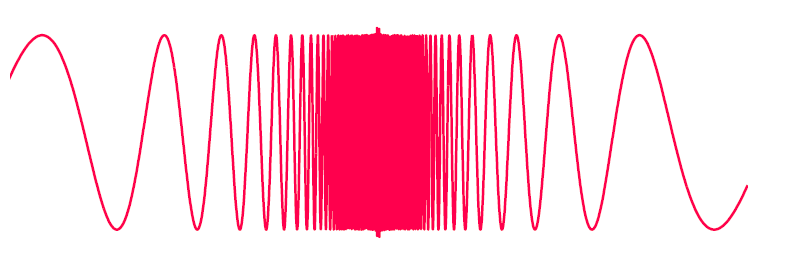
\includegraphics[0.8]{sin.png}
    
    $f(x) = sin(10/x), n=10^6$, se plotean 2000 puntos cerca del origen. %Fijense que en el anterior, si quier
\end{frame}

%TODO hablar de la primera formula baricentrica y contar como se llega a la segunda
%TODO dar una intuiciion de la estabilidad
%TODO expresar distinta la formula baricentrica que es un asco asi


% Les quiero hablar un poquito de otra manera de aproximar funciones con polinomios


\begin{frame}

    % Chebychev no minimiza realmente el error, sino W(x)
    \begin{Teorema}[Equioscilación]
    Sea $f :[a,b] \rightarrow \mathbb{R}$ una función continua y $g$ un polinomio de grado menor o igual a $n$. Entonces, son equivalentes: \bigskip
    
    1) Entre todos los polinomios de grado $\leq n$, $g$ minimiza $||f -g ||_\infty$ \bigskip
    
    2) Existen $n+2$ puntos $a \leq x_0 \leq x_1 \leq ... \leq x_{n+1} \leq b$ tal que $f(x_i) - g(x_i) = \sigma\ (-1)^i  ||f -g ||_\infty$, con $\sigma = \pm 1$.\end{Teorema} \bigskip
    
    A $g$ se lo suele llamar la mejor aproximación de $f$, y es costoso computarla.
    
    % Hacer dibujito de la norma infinito!
    % Recordar qué es lo que minimiza interpolar en los ceros de Chebyschev
    
    \end{frame}

\begin{frame}{¿Qué es mejor?}

% Decir oralmente que se puede probar que el error de uno no se aleja mucho del error del otro

¿Qué conviene? ¿Usar la mejor aproximación o la fórmula baricéntrica en los polinomios de Chebyschev?

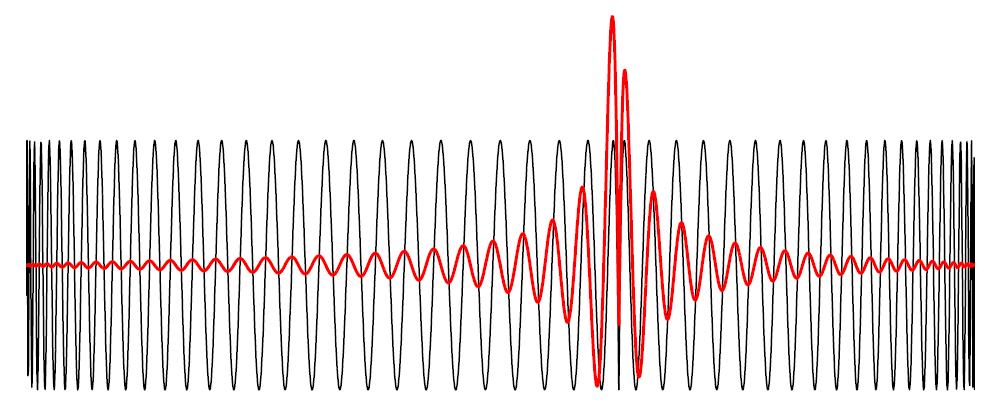
\includegraphics[scale=0.5]{comparacion.png}

$f(x) = |x-1/4|$, $x\in[-1,1], n = 100$ \\
En negro: error de la mejor aproximación \\
En rojo: error en los puntos de Chebyshev

\end{frame}

\begin{frame}

Referencias: \bigskip
\begin{itemize}
    \item \href{run:./file.txt}{File.txt}   "Six Myths of Polynomial Interpolation and
Quadrature" (Trefethen, 2011) \url{https://people.maths.ox.ac.uk/trefethen/publication/PDF/2011_139.pdf}
    \item Barycentric Lagrange Interpolation, (Berrut y Trefethen, 2004) \url{goo.gl/qZAjQ9}
    \item The numerical stability of barycentric Lagrange
interpolation (Higham, 2004) \url{goo.gl/UfbGf1}
\end{itemize}
\end{frame}

\end{document}
